\usepackage{amsmath}
\usepackage{tikz}
\usetikzlibrary{arrows.meta,
                calc, chains,
                decorations.pathreplacing,
                calligraphy,% had to be after decorations.pathreplacing
                positioning,
                math}
\makeatletter
% the contents of \squarecorner were mostly stolen from pgfmoduleshapes.code.tex
\def\squarecorner#1{
    % Calculate x
    %
    % First, is width < minimum width?
    \pgf@x=\the\wd\pgfnodeparttextbox%
    \pgfmathsetlength\pgf@xc{\pgfkeysvalueof{/pgf/inner xsep}}%
    \advance\pgf@x by 2\pgf@xc%
    \pgfmathsetlength\pgf@xb{\pgfkeysvalueof{/pgf/minimum width}}%
    \ifdim\pgf@x<\pgf@xb%
        % yes, too small. Enlarge...
        \pgf@x=\pgf@xb%
    \fi%
    % Calculate y
    %
    % First, is height+depth < minimum height?
    \pgf@y=\ht\pgfnodeparttextbox%
    \advance\pgf@y by\dp\pgfnodeparttextbox%
    \pgfmathsetlength\pgf@yc{\pgfkeysvalueof{/pgf/inner ysep}}%
    \advance\pgf@y by 2\pgf@yc%
    \pgfmathsetlength\pgf@yb{\pgfkeysvalueof{/pgf/minimum height}}%
    \ifdim\pgf@y<\pgf@yb%
        % yes, too small. Enlarge...
        \pgf@y=\pgf@yb%
    \fi%
    %
    % this \ifdim is the actual part that makes the node dimensions square.
    \ifdim\pgf@x<\pgf@y%
        \pgf@x=\pgf@y%
    \else
        \pgf@y=\pgf@x%
    \fi
    %
    % Now, calculate right border: .5\wd\pgfnodeparttextbox + .5 \pgf@x + #1outer sep
    \pgf@x=#1.5\pgf@x%
    \advance\pgf@x by.5\wd\pgfnodeparttextbox%
    \pgfmathsetlength\pgf@xa{\pgfkeysvalueof{/pgf/outer xsep}}%
    \advance\pgf@x by#1\pgf@xa%
    % Now, calculate upper border: .5\ht-.5\dp + .5 \pgf@y + #1outer sep
    \pgf@y=#1.5\pgf@y%
    \advance\pgf@y by-.5\dp\pgfnodeparttextbox%
    \advance\pgf@y by.5\ht\pgfnodeparttextbox%
    \pgfmathsetlength\pgf@ya{\pgfkeysvalueof{/pgf/outer ysep}}%
    \advance\pgf@y by#1\pgf@ya%
}
\makeatother

\pgfdeclareshape{square}{
    \savedanchor\northeast{\squarecorner{}}
    \savedanchor\southwest{\squarecorner{-}}

    \foreach \x in {east,west} \foreach \y in {north,mid,base,south} {
        \inheritanchor[from=rectangle]{\y\space\x}
    }
    \foreach \x in {east,west,north,mid,base,south,center,text} {
        \inheritanchor[from=rectangle]{\x}
    }
    \inheritanchorborder[from=rectangle]
    \inheritbackgroundpath[from=rectangle]
}

\definecolor{NNGreen}{RGB}{38, 222, 129}
\definecolor{NNBlue}{RGB}{55, 66, 250}
\definecolor{NNBlack}{RGB}{47, 53, 66}
\definecolor{NNYellow}{RGB}{241, 196, 15}
\definecolor{NNRed}{RGB}{255, 107, 107}
\begin{document}
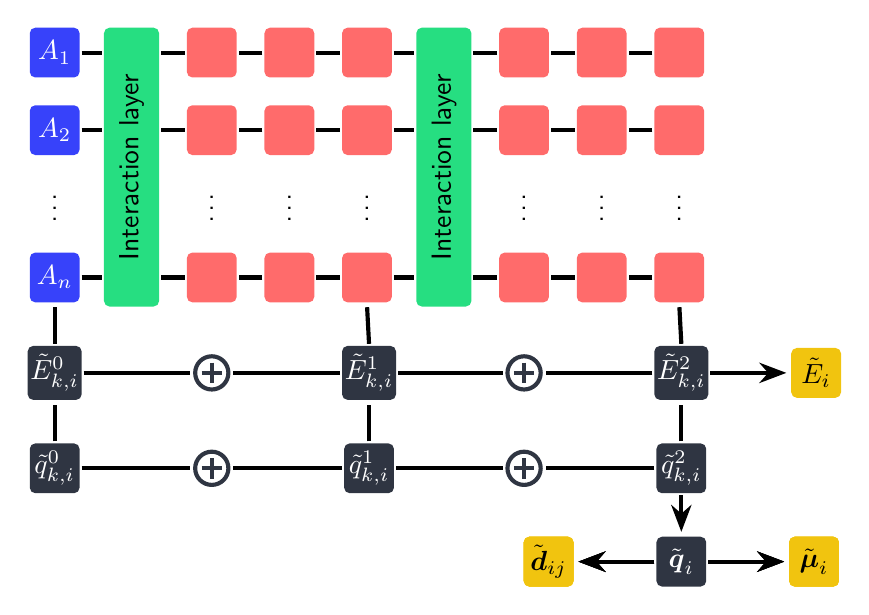
\begin{tikzpicture}[
    font = \sffamily,
    shorten > = 1pt,
    > = Stealth,
    line width = 1.5pt,
    start chain = going below,
    neuron/.style = {
      square,
      fill=#1,
      minimum size= 18pt,
      inner sep = 1pt,
      rounded corners=2pt,
    },
  ]

    % total number of rows, including the "..." row
    \pgfmathsetmacro\nrows{4};
    % number of interaction layers
    \pgfmathsetmacro\nint{2};
    % number of on-site layers
    \pgfmathsetmacro\natom{3};
    % index of the row being "..."
    \pgfmathsetmacro\idots{int(\nrows-1)};

    % draw the input layer
    \foreach \i in {1, ..., \nrows} {
      \ifnum \i = \idots
        % "..." row
        \node[neuron=white, on chain, below=2mm] (n-1-\i) {$\vdots$};
      \else
        \ifnum \i = \nrows
          \pgfmathsetmacro\idx{"n"};
        \else
          \pgfmathsetmacro\idx{\i};
        \fi
        \node[neuron=NNBlue, on chain, below=3mm] (n-1-\i) {\color{white}$A_\idx$};
      \fi
    }
    % draw first hierarchical output
    \node[neuron=NNBlack, on chain, below=5mm] (e-1) {\color{white}$\tilde{E}_{k,i}^0$};
    \node[neuron=NNBlack, below=5mm of e-1] (q-1) {\color{white}$\tilde{q}_{k,i}^0$};
    \foreach \i in {1, ..., \nint} {
      \pgfmathsetmacro\blockidx{int((\i - 1) * \natom + 1)};
      % Interaction layer i
      \path   let \p1 = ($(n-\blockidx-1.north) - (n-\blockidx-\nrows.south)$),
                  \n\i = {veclen(\y1,\x1)} in
              node (r\i) [
                minimum height=\n\i,
                minimum width=7mm, fill = NNGreen,
                below right=0mm and 6 mm of n-\blockidx-1.north,
                rounded corners=2pt
              ]{\rotatebox{90}{Interaction layer}};
      % atom layers
      \foreach \j in {1, ..., \natom} {
        \pgfmathsetmacro\nodeidx{int(\blockidx + \j)};
        \ifnum \j = 1
          \pgfmathsetmacro\parent{"r\i"};
        \else
          \pgfmathsetmacro\parentidx{int(\nodeidx - 1)};
          \pgfmathsetmacro\parent{"n-\parentidx-1"};
        \fi
        \foreach \k in {1, ..., \nrows} {
          \ifnum \k = \idots
            \node[neuron=white, right=3mm of n-1-\k -| \parent.east] (n-\nodeidx-\k) {$\vdots$};
          \else
            \node[neuron=NNRed, right=3mm of n-1-\k -| \parent.east] (n-\nodeidx-\k) {};
            \draw[-] (n-\nodeidx-\k) -- (n-1-\k -| \parent.east) ++ (0.5,0);
          \fi
        }
      }
      % hierarchical outputs
      \pgfmathsetmacro\parent{int(\i * \natom)};
      \pgfmathsetmacro\nodeidx{int(\i + 1)};
      % draw node
      \node[neuron=NNBlack, right=3mm of e-1 -| n-\parent-\nrows.east] (e-\nodeidx) {\color{white}$\tilde{E}_{k,i}^\i$};
      \node[neuron=NNBlack, below=5mm of e-\nodeidx] (q-\nodeidx) {\color{white}$\tilde{q}_{k,i}^\i$};
    }
    % final output
    \pgfmathsetmacro\nlayers{int(\nint + 1)}
    \pgfmathsetmacro\out{int(\nint + 2)}
    % draw node
    \node[neuron=NNYellow, right=10mm of e-\nlayers] (e-\out) {\color{black}$\tilde{E}_i$};
    \node[neuron=NNBlack, below=5mm of q-\nlayers] (q-\out) {\color{white}$\tilde{\boldsymbol{q}}_i$};

    % rest nodes connections
    % input to first interaction
    \foreach \i in {1, ..., \nrows} {
      \ifnum \i = \idots
      \else
        \draw[-] (n-1-\i) -- (n-1-\i.east -| r1.west) ++ (0.5,0);
      \fi
    }
    % atom to second interaction
    \foreach \i in {2, ..., \nint} {
      \pgfmathsetmacro\atom{int((\i - 1) * \natom + 1)}
      \foreach \j in {1, ..., \nrows} {
        \ifnum \j = \idots
        \else
          \draw[-] (n-\atom-\j) -- (n-1-\j.east -| r\i.west) ++ (0.5,0);
        \fi
      }
    }
    % all hierarchical outputs
    \foreach \i in {0, ..., \nint} {
      % to each atom layer
      \pgfmathsetmacro\outidx{int(\i + 1)}
      \pgfmathsetmacro\atomidx{int(\i * \natom + 1)}
      \draw[-] (e-\outidx.north) -- (n-\atomidx-\nrows.south);
      % from e hierarchical to q hierarchical
      \draw[-] (q-\outidx.north) -- (e-\outidx.south);
      % a "plus" node between hierarchical outputs
      \ifnum \i > 0
        \pgfmathsetmacro\atomidx{int((\i - 1) * \natom + 2)}
        % draw a bare circle
        \node[circle, minimum size=12pt, draw=NNBlack, at = (e-1 -| n-\atomidx-1)] (pe-\i) {};
        % draw the plus sign
        \node[
          circle, minimum size=8pt, at = (e-1 -| n-\atomidx-1),
          path picture={
        \draw[NNBlack] (path picture bounding box.west)+(1pt,0) -- (path picture bounding box.east); 
        \draw[NNBlack] (path picture bounding box.north)+(0,-1pt) -- (path picture bounding
        box.south); 
          }
        ] () {};
        \draw[-] (e-\outidx) -- (pe-\i);
        \draw[-] (e-\i) -- (pe-\i);
        % for charges
        \node[circle, minimum size=12pt, draw=NNBlack, at = (q-2 -| n-\atomidx-1)] (pq-\i) {};
        \node[
          circle, minimum size=8pt, at = (q-2 -| n-\atomidx-1),
          path picture={
        \draw[NNBlack] (path picture bounding box.west)+(1pt,0) -- (path picture bounding box.east); 
        \draw[NNBlack] (path picture bounding box.north)+(0,-1pt) -- (path picture bounding
        box.south); 
          }
        ] () {};
        \draw[-] (q-\outidx) -- (pq-\i);
        \draw[-] (q-\i) -- (pq-\i);
      \fi
      % last hierarchical to final output
      \ifnum \i = \nint
        \pgfmathsetmacro\last{int(\outidx + 1)}
        \draw[->] (e-\outidx) -- (e-\last);
        \draw[->] (q-\outidx) -- (q-\last);
      \fi
      \pgfmathsetmacro\outidx{int(\nint + 1)}
      \pgfmathsetmacro\last{int(\nint + 2)}
      \node[neuron=NNYellow, right=10mm of q-\last] (mu) {\color{black}$\tilde{\boldsymbol{\mu}}_i$};
      \node[neuron=NNYellow, left=10mm of q-\last] (nacr) {\color{black}$\tilde{\boldsymbol{d}}_{ij}$};
      \draw[->] (q-\last) -- (mu);
      \draw[->] (q-\last) -- (nacr);
    }
\end{tikzpicture}